\section{Organigramme des t�ches}


\subsection{Macro-phasage}

Les approches organisation et produit du macro-phasage �tant d�taill�es
dans les deux parties pr�c�dentes, on s'attardera ici plus pr�cis�ment sur
l'approche activit�.
A chaque livrable est associ� un plan (sommaire du dossier correspondant) ; � chaque partie majeure
correspond une t�che. En fonction de son importance cette t�che peut �tre
associ�e � une ou plusieurs personnes. Enfin certaines t�ches correspondant
� une activit� de brainstorming sont associ�es � l'ensemble de l'�quipe.


\subsection{Planning pr�visionnel}

Le planning est r�alis� depuis la semaine 52 de l'ann�e 2010 jusqu'� la
semaine 3 de l'ann�e 2011. Les semaines comportant deux s�ances de travail
sont d�doubl�es (par exemple : S2.1 et S2.2) dans le planning. Enfin, on
distingue les deux phases du projet au niveau des livrables et au niveau
des semaines de travail.\\

\begin{center}
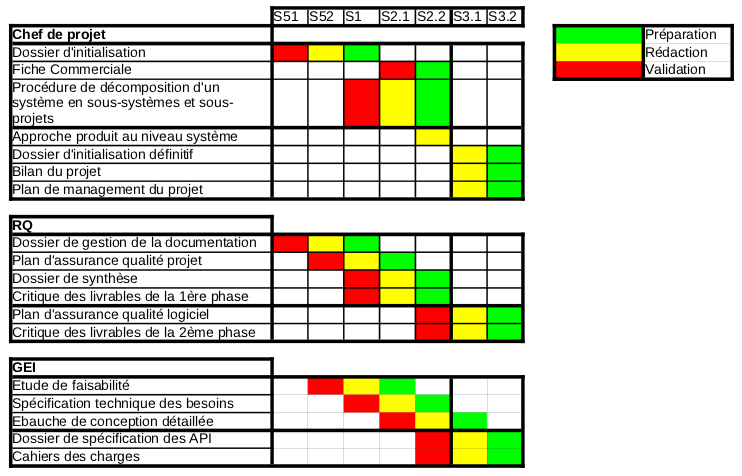
\includegraphics[scale=0.8]{\PIXPATH/planning}
\end{center}
